\section{Design of the Protocol}
\label{sec:insecure-design}

The Insecure CC Protocol uses the NFC channel to transmit messages between the credit card and the point of sale.
This decision is based on the following factors:
\begin{itemize}
\item NFC is a wireless channel, and thus it is unaffected by card demagnetization or read errors due to dirty or corroded contacts.
\item NFC has a very short range (under 10 cm), mitigating many of the privacy concerns commonly associated with wireless channels.
\item NFC supports communication with unpowered (termed ``passive'') devices, allowing the credit card to forego having its own power source.
\item Even passive NFC devices such credit cards can perform complex computation while being wirelessly powered by the point of sale.
\end{itemize}

In the Insecure CC Protocol, the customer indicates his intention to pay by enabling communication between the point of sale and the NFC credit card.
This is done by the customer bringing the credit card within range of the point of sale (no more than 4 centimeters away).
Once within range of each other, the point of sale may send messages to the credit card and receive any resulting responses.
The steps involved in this protocol, illustrated in Figure \ref{fig:insecure-ccp}, are as follows:

\begin{enumerate}
\item The point of sale displays the price of the purchase on its screen, while simultaneously attempting to establish communication over NFC.
\item If the customer agrees with the displayed price, he brings his credit card within 4 centimeters of the point of sale and communication between the point of sale and the credit card is established.
\item The point of sale sends a Solicitation message to the credit card.
\item The credit card responds to the solicitation message with a Card Information message, supplying the point of sale with the necessary information to initiate a transaction,
	and identifying the credit card's issuing bank.
\item Then the point of sale sends a Charge Request message to the bank. This message is sent securely over the Internet.
\item The bank verifies the details of the charge request, and responds to the point of sale with a Approval message, indicating whether the Charge Request has been accepted.
\end{enumerate}


\begin{figure}
  \caption{The Insecure CC Protocol}
  \centering
    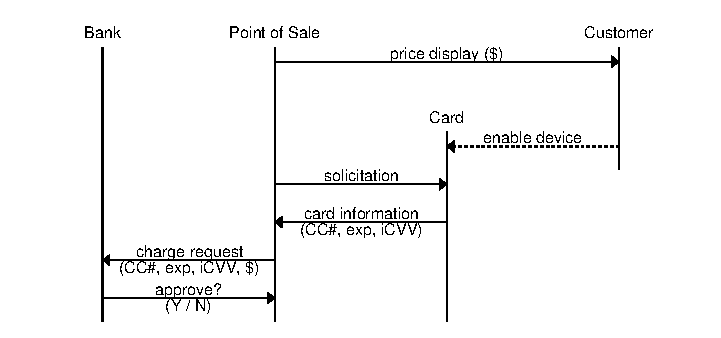
\includegraphics{img/insecure_ccp.eps}
  \label{fig:insecure-ccp}
\end{figure}

The message contents in the Insecure CC Protocol are as follows:

\begin{description}

\item[Solicitation:]
In practice, the solicitation message actually consists of a number of messages sent in both directions.
The purpose of these messages is to exchange information about the credit card type (e.g. \emph{Visa Credit}) and the point of sale model (e.g. \emph{2PAY.SYS.DDF01}), which defines the format of subsequent messages.
It is a choreographed dance with a specific (and constant) set of messages for a given model of point of sale and credit card, so we abstract this conversation to a single solicitation message.

\item[Card Information:]
This message contains all information necessary to coordinate an arbitrary charge request to the credit card's issuing bank. It consists of four components:
\begin{itemize}
	\item The credit card number, identical to the number printed on the front of the card.
	\item The credit card's expiration date.
	\item An \emph{iCVV} (``integrated Card Verification Value'').
		This iCVV is a security code, similar to the 3-digit number printed on the back of a credit card, but is newly generated for each transaction.
		It is an element in a pseudo-random sequence generated by a secret seed known only to the credit card and its issuing bank, making it unpredictable to third parties.
	\item The issuing bank name.
		This field is used for routing purposes, and is not a component of the subsequent charge request.
		As such, it is not pictured in Figure \ref{fig:insecure-ccp}.
\end{itemize}

\item[Charge Request:]
This message is sent to the bank identified in the card information message, and consists of four components:
\begin{itemize}
	\item The credit card number, identifying the account to be charged.
	\item The credit card's expiration date.
	\item The credit card's iCVV.
	\item The dollar amount to be charged.
\end{itemize}

\item[Approval:]
This message consists of a \emph{response code} determined by the bank, indicating its decision relating to the charge request.
The bank makes this decision after verifying the information supplied in the charge request message, and performing additional checks such as matching the purchase to a known location of the customer.
The most common response codes are the result of a simple approval decision (i.e. ``Approved'' or ``Declined''),
although a number of different codes (e.g. ``Pick up card'' if the card was reported lost or stolen, etc.) are also supported.
We abstract this message as a single bit: whether or not the customer's account has been charged.

\end{description}
